\section{GMSE Systems Architecture}

The objective of this section is to decompose the components of the simulation program from a high-level description and
interconnectivity of its components to low-level technical constructs of essential components of GMSE. As simulation
programs are no simple task to implement, multiple components emerge to address specific tasks. At a systems level,
these modules must then interact in such a fashion to achieve the overall goal: avionics simulation.

An effective top-down method of presenting the taxonomy of architectures is as described in \cite{levis_c4isr_2000}. The
work breaks systems down into three architectures: operational architecture, a systems architecture, and a technical
architecture. The operational architecture describes what the system does by describing how each of the packages perform
and how they are integrated together, the systems architecture states the major subsystems and how they behave, and the
technical architecture provides the details of each subsystem. In the following sections the operational, systems, and
technical architectures are presented in \autoref{sec:gmse-operational-architecture},
\autoref{sec:gmse-systems-architecture}, and \autoref{sec:gmse-technical-architecture}, respectively, for the GMSE. The
primary focus of this work is to deconstruct GMSE, the other components that interact with GMSE provide essential
insight into the constructs of GMSE. As such, description where required for external modules will be provided.

\subsection{Operational Architecture}
\label{sec:gmse-operational-architecture}

When describing a large piece of software, one can often decompose the software into a set of packages. Packages
describes software that are composed of multiple modules which ideally are designed to perform a specialized
task\footnote{This process can be extended ad nauseam to further and further decompose items until its most primitive
forms are derived. That will be avoided as much as possible to keep the discussion relevant to the critical
components.}. At the subsystem level, there are three main packages: Core Avionics\footnote{Often times modules
associated with core avionics are also referred to as subsystems}, External Sensors and Modules, and the GMSE. The
modules and their interconnectivity is shown in \autoref{fig:gmse-operational-architecture}.

The core avionics package describes the suite of software being developed that that has immediate agency to the behavior
of the avionics system. For example, the Avionics Data Computer (ADC) is the ``brain'' of the avionics system. It
contains the vehicle's perceived external state as well as its internal operating state. It also supplies flow of data
at the correct rate to the correct system. The Flight Control Module (FCM) utilizes the data from the ADC to assist in
maintaining stability and controlling the vehicle to the waypoints described by the planning algorithms utilized by the
Flight Navigation Module (FNC).

For the core avionics to function in the real world, a sense of the vehicle's immediate surroundings must be established
via various sensors and external modules. In particular, the sensors (more often than not) are off-the-shelf products
that require integration with the core avionics. The sensors in this package may contain software modules either that
mimic the behavior of a sensor, or include the physical sensor in-the-loop of the simulation. This software package also
contains ``external modules'' which are other off-the-shelf components that require integration into the core avionics. As
an example, if one desires to incorporate data linking to transfer data in real-time to a base station, the physical
device to transfer the data via radio frequency (RF) would be included as an ``external module''.

The objective of the GMSE package is to drive both the sensor modules and core avionics by spawning all the necessary
processes, executing tasks at their scheduled times, calculating the ``state of the world'', calculating the state of
``ownship'', as well as data logging and plotting. That is, the objective of GMSE is to provide all the ``services''
that would otherwise have been provided by real-world scenarios. The means of connectivity between each of the packages
is provided by the Small Dynamic Subsystem Interface Protocol (SDSIP). A description of the communications is provided
in \autoref{sec:sdsip}.

\begin{figure*}[ht]
  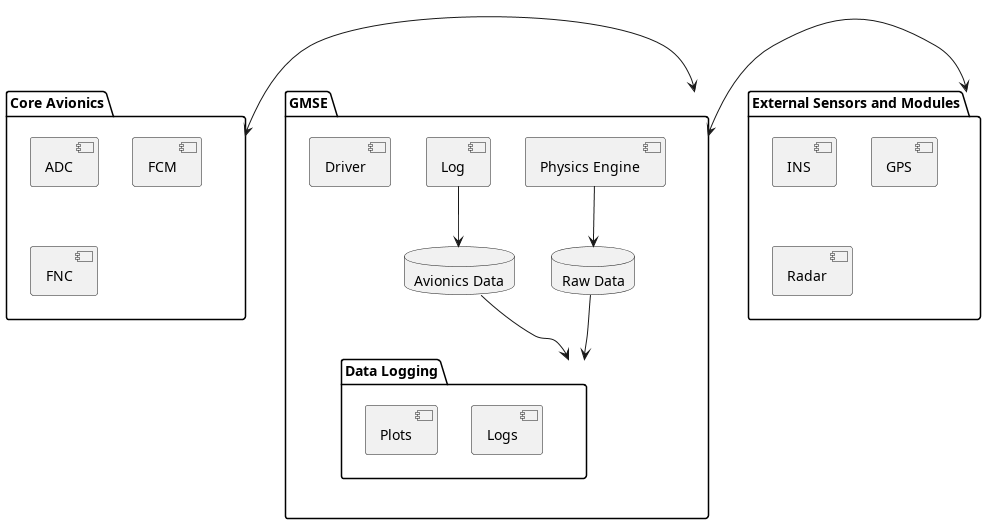
\includegraphics[width=\textwidth]{gmse-operational-architecture}
  \caption{Operational architecture for GMSE. The core avionics and external sensors and modules packages are included
    to depict the flow of data (indicated by the arrows). The GMSE package is composed of the driver, logger, physics
    engine, various databases, and the data logging modules. The driver module does the initialization, spawns the
    necessary processes, and executes the mock sensors and modules. The logger ``sniffs'' the data being transferred and
    stores it in the appropriate databases. The avionics data is the information that would be transmitted within the
    avionics systems and the raw data is the information generated by the sensors and external modules. The physics
    engine is the crux of the simulation by propagating the ``world'' and calculating all forces applied to the
    vehicle.}
  \label{fig:gmse-operational-architecture}
\end{figure*}

\subsection{Systems Architecture} \label{sec:gmse-systems-architecture}

The GMSE package consists of several packages as depicted in \autoref{fig:gmse-operational-architecture}. These modules
are the GMSE driver, logger, and physics engine. The driver module is the part of the GMSE package that initializes the
simulation, spawns all the required processes, and ensures the correct modeled external modules and sensors are updated
at the correct times. The logging module of the GMSE package inputs both the avionics data and the raw data created by
the physics engine. The physics engine module is the back end that models the world components such as the physical
location of the aircraft, wind and other disturbances, as well as obstacles. Each of these packages are to be described
in further detail in the subsequent sections.

\subsubsection{GMSE Driver}

The GMSE driver is the core of the GMSE. The driver package provides the following functionality:

\begin{enumerate}
  \item Initialization
    \begin{itemize}
      \item SDSIP (i.e. communications package),
      \item initialize the state of the ``world'', and
      \item initialize the state of ``ownship''
    \end{itemize}
  \item Spawn
    \begin{itemize}
      \item GMSE physics engine
      \item sensor and external modules and
      \item core avionics
    \end{itemize}
  \item Execution
    \begin{itemize}
      \item GMSE loggers,
      \item GMSE physics engine, and
      \item mock sensor modules
    \end{itemize}
\end{enumerate}

Beginning with the initialization process, the GMSE driver module is meant to provide all the information that the
simulation requires to function. The initialization begins by executing SDSIP to generate the required code to interface
with the ``device drivers'', publishers, and subscribers. The initialization process is as described in
\autoref{sec:sdsip}. The GMSE driver also provides the required parameters to the physics engine so that it can
initialize the ``state of the world''. That is, there exist YAML files specifying positional factors such as initial
coordinate frames positions and orientations, and obstacle locations and dimensions. There exist other YAML files
specifying the physical aspects such as wind speeds and directions, as well as physical parameters to describe the
behavior of the avionics systems being modeled. The core avionics must be initialized so that the ``world state'' aligns
with the ``ownship'' state (i.e. the positioning and sensing done by the simulated avionics is consistent with the
physics engine world state). As an example, if one desires to test flight maneuvers, one may wish to initialize the
system in a way that allows the vehicle to perform the maneuver promptly (i.e. mid-flight at a specified speed and
altitude to perform a loop).

After initialization has been completed, the GMSE driver process begins to spawn processes and threads required to
execute the simulation process. The physics engine is created as that is the package that propagates and maintains the
current state of the ``world''. The sensors and external modules are then created to be able to ``perceive'' the world
from the vehicle's perspective. Finally, the core avionics is created.

With all the required packages instantiated, now the simulation may begin execution. The physics engine is executed
first to propagate the state of the world and ownship forward by a some discrete step size. The sensors and external
modules are then provided the ``world state'' data which is then the core avionics may utilize. It is important to note
that the core avionics is not included in the execution. That is, while the core avionics process is spawned from the
driver module during the ``spawn'' phase, it is not being driven by GMSE. In other words, the core avionics is spawned
as a sub-process that is executing independently of GMSE. This is done to simulate as if the core avionics were embedded
on a physical system that is merely receiving external inputs.

In the following sections, further description about the systems architecture for each of the packages is provided.

\subsubsection{GMSE Logger}

The GMSE logger maintains the responsibility of ``sniffing'' all the traffic that is generated from the physics engine
and transmitted via SDSIP and storing them in respective databases labeled ``raw'' and ``avionics'' data, respectively.
In other words, the GMSE logger acts both as a flight recorder for both the simulated vehicle and for the physics
engine. Both pieces of data are logged in their respective databases so that the raw data generated by the physics
engine (i.e. the input) can be compared to the resulting avionics response (i.e. the output).

Once the data has been written to their respective databases, generic or custom plotting or logging modules may be
written to glean information on what the physics engine is generating as well as monitor the real-time behavior of the
avionics system.

\subsubsection{GMSE Physics Engine}

The physics engine can be thought of as the ``back end'' of the GMSE. The physics engine can be implemented utilizing
various different methods, such as polynomial models, multipoint models, and tabular models
\cite{banks_discussion_nodate}. However, regardless of how any particular model may maintain the world state internally,
certain information must be exposed in a general manner such that the sensing modules may be able to retrieve its
required information from the ``world''. Such information, while not exhaustive, includes: airspeed, yaw, pitch,
altitude, etc. The physics engine is also responsible for estimating the forces applied to the vehicle. These forces
will then in turn alter the vehicles position, velocity, and acceleration vectors forcing a response from the core
avionics system.

\subsubsection{GMSE Driver}

The GMSE driver can be thought of the ``glue'' that holds all the pieces together. The driver package is responsible for
ensuring all the required executables are running, initializing each package with the appropriate data, and providing
the required data to the sensing and external modules at the correct time and, in turn, providing the data to the core
avionics in a timely manner.

The external sensors and modules are instantiated as threads from the GMSE driver. These processes are created in this
manner because GMSE is in charge of the timing in which these components are executed, but it is desired that when they
run, these modules run independently to GMSE so that timing requirements are met. This is juxtaposed to the core
avionics being instantiated as a separate process. The core avionics being run as a separate process is meant to enforce
the fact that the core avionics is disjoint from GMSE, and to further emphasize that the core avionics is acting only on
the inputs that would be received during operation.

\subsection{Technical Architecture} \label{sec:gmse-technical-architecture}
